% Created 2013-10-05 Sat 01:18
\documentclass[bigger]{beamer}
\usepackage[utf8]{inputenc}
\usepackage{hyperref}
\usepackage{graphicx}
\usepackage{longtable}
\usepackage{float}
\mode<beamer>{\usetheme{Madrid}}
\usepackage{verbatim}
\usepackage{color}
\usepackage{amsmath,amsfonts,amssymb}
\AtBeginSection[]{\begin{frame}<beamer>\frametitle{Topic}\tableofcontents[currentsection]\end{frame}}
\providecommand{\alert}[1]{\textbf{#1}}

\title{Climate Change Health Impact Assessments:  Farmer Suicide and Drought Case Study.}
\author{Ivan Hanigan$^1$, David Fisher$^2$, Steven McEachern$^3$}
\date{\today}
\hypersetup{
  pdfkeywords={},
  pdfsubject={},
  pdfcreator={Emacs Org-mode version 7.9.3f}}

\institute[NCEPH]{$^1$National Centre for Epidemiology and Population Health (ANU) \\ $^2$Information Technology Services (ANU) \\ $^3$Australian Data Archives (ANU)}
\begin{document}

\maketitle

% Org-mode is exporting headings to 3 levels.

\section{Aim}
\label{sec-1}
\begin{frame}
\frametitle{Aim}
\label{sec-1-1}

Climate Change Health Impact Assessments (CCHIA) need
\begin{itemize}
\item Workflow tools for data management and analysis
\item Enhanced capacity for experimentation, reviews, revisions
\end{itemize}

General approach:
\begin{itemize}
\item historical exposure-response functions, control covariates
\item future response with changed exposures and population at risk
\end{itemize}
\end{frame}
\begin{frame}
\frametitle{Motivating Case Study: Climate/Suicide}
\label{sec-1-2}

\begin{itemize}
\item Suicide has been linked to climate in a variety of studies
\item Climate change impact on mental health is a gap in knowledge
\item Use methods to analyse the relationship between Drought/Suicide
\item Estimate future Climate Change impacts
\end{itemize}
\end{frame}
\begin{frame}
\frametitle{New Tools are Needed}
\label{sec-1-3}

\begin{itemize}
\item Restrictions on access to suicide data have increased recently.
\item Growing concern about the \textbf{Replicability Crisis}, (Peng 2011, \emph{Science}, 334).
\item Access to data and analytic software addresses this.
\item We built a safe Sever/Client IT environment.
\end{itemize}
\end{frame}
\section{Methods}
\label{sec-2}
\begin{frame}
\frametitle{System Design}
\label{sec-2-1}

\begin{figure}[!h]
\centering
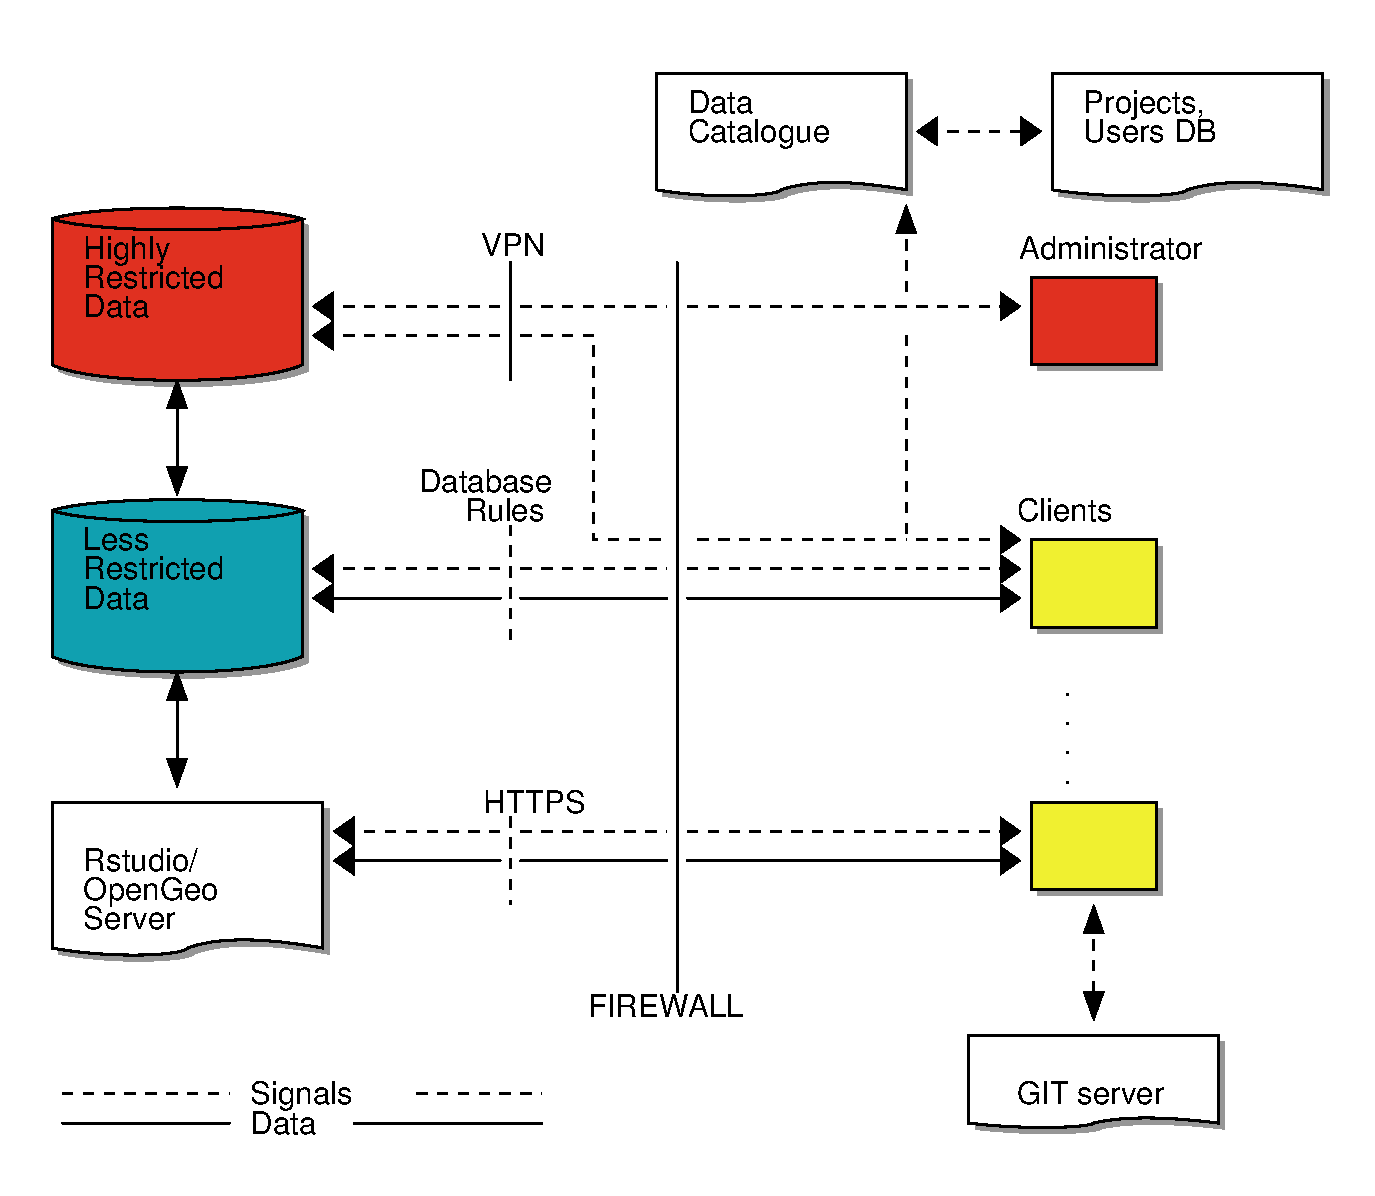
\includegraphics[width=.65\textwidth]{opensoft.pdf}
\caption{1. System Design}
\label{fig:sys}
\end{figure}
\end{frame}
\begin{frame}
\frametitle{Linux Cluster}
\label{sec-2-2}

\begin{itemize}
\item National Research Cloud (www.nectar.org.au/research-cloud)
\item Centos 6.4 (www.centos.org)
\end{itemize}
\end{frame}
\begin{frame}
\frametitle{PostGIS Database (The Brawn)}
\label{sec-2-3}

\begin{itemize}
\item PostgreSQL 9.2 (www.postgresql.org)
\item PostGIS 2.0 (postgis.refractions.net)
\end{itemize} 
\end{frame}
\begin{frame}
\frametitle{Analysis (The Brains)}
\label{sec-2-4}

\begin{itemize}
\item R language for statistical computing (www.r-project.org)
\item Rstudio server (www.rstudio.com/)
\item OpenGeo Suite (opengeo.org)
\end{itemize}
\end{frame}
\begin{frame}
\frametitle{Information Management}
\label{sec-2-5}

\begin{itemize}
\item Projects,UsersDB Oracle XE APEX (www.oracle.com)
\item Data Catalogue (assda.anu.edu.au/ddiindex.html)
\end{itemize}
\end{frame}
\begin{frame}
\frametitle{The Client Side}
\label{sec-2-6}

\begin{itemize}
\item The Kepler Project (www.kepler-project.org)
\item pgAdmin (www.pgadmin.org)
\item Git Version Control and GitHub (github.com)
\end{itemize}
\end{frame}
\begin{frame}
\frametitle{Case Study: Historical}
\label{sec-2-7}

\begin{footnotesize}
\begin{itemize}
\item {\color{red}Restricted Health and Drought data} and 
\item {\color{blue}Less Restricted Population data} 
\end{itemize}
(Colours refer to data storage and access rules shown in Figure 1).
\begin{eqnarray*}
        log({\color{red} O_{ijk}})  & = & s({\color{red}ExposureVariable})  + {\color{blue} OtherExplanators}  \\
        & &   + AgeGroup_{i} + Sex_{j} \\
        & &   + {\color{blue} SpatialZone_{k}}  \\
        & &  + sin(Time \times 2 \times \pi) + cos(Time \times 2 \times \pi) \\
        & &  + Trend \\
        & &   + offset({\color{blue} log(Pop_{ijk})})\\
\end{eqnarray*}
\end{footnotesize}
\begin{tiny}
\noindent Where:\\
        \indent ${\color{red}O_{ijk}}$ = Outcome (counts) by Age$_{i}$, Sex$_{j}$ and SpatialZone$_{k}$ \\
        \indent {\color{red}ExposureVariable} = Data with {\color{red}Restrictive Intellectual Property~(IP)} \\
        \indent {\color{blue}OtherExplanators} = Other {\color{blue}Less Restricted}  Explanatory variables \\
        \indent s( ) = penalized regression splines \\
        \indent ${\color{blue} SpatialZone_{k}}$  = {\color{blue} Less Restricted} data representing the $SpatialZone_{k}$  \\
        \indent Trend = Longterm smooth trend(s) \\
        \indent ${\color{blue}Pop_{ijk}}$ = interpolated Census populations, by time in each group\\
\end{tiny}
\end{frame}
\begin{frame}
\frametitle{Case Study: Historical}
\label{sec-2-8}

Hanigan et al, 2012, \emph{PNAS}, 109:
\begin{itemize}
\item 38 years suicide rates with drought by 11 regions, age and sex
\item Estimated 9\% in rural males aged 30-49 due to drought over the period
\item Increased for rural males 10-29 y
\item Association with hot temp + spring
\end{itemize}
\end{frame}
\begin{frame}
\frametitle{Case Study: Future}
\label{sec-2-9}

Bambrick et al, 2008, Garnaut Review:
\begin{footnotesize}
$$Y_{ijk}=\sum_{lm}(e^{(\beta_{ijk} \times {\color{red} X_{lm}})} - 1) \times {\color{red}BaselineRate_{jkl}} \times {\color{blue} Population_{jklm}}$$
\noindent Where:\\
$\beta_{ijk}$ = the ExposureVariable coefficient for zone$_i$, age$_j$ and sex$_{k}$ \\
${\color{red}X_{lm}}$ = Projected Future ExposureVariables {\color{red} with Restrictive IP} \\
{\color{red}BaselineRate$_{jkl}$} = {\color{red}avgDeathsPerTime}/{\color{blue}avgPopPerTime} in age$_j$, sex$_k$ and zone$_l$ \\
{\color{blue}Population$_{jklm}$} = projected populations by age$_j$, sex$_k$, zone$_l$ and time$_m$ {\color{blue} (With Less Restrictions)}\\

\end{footnotesize}
\end{frame}
\section{Results}
\label{sec-3}
\begin{frame}
\frametitle{Drought-suicide response function}
\label{sec-3-1}

\begin{figure}[!h]
\centering
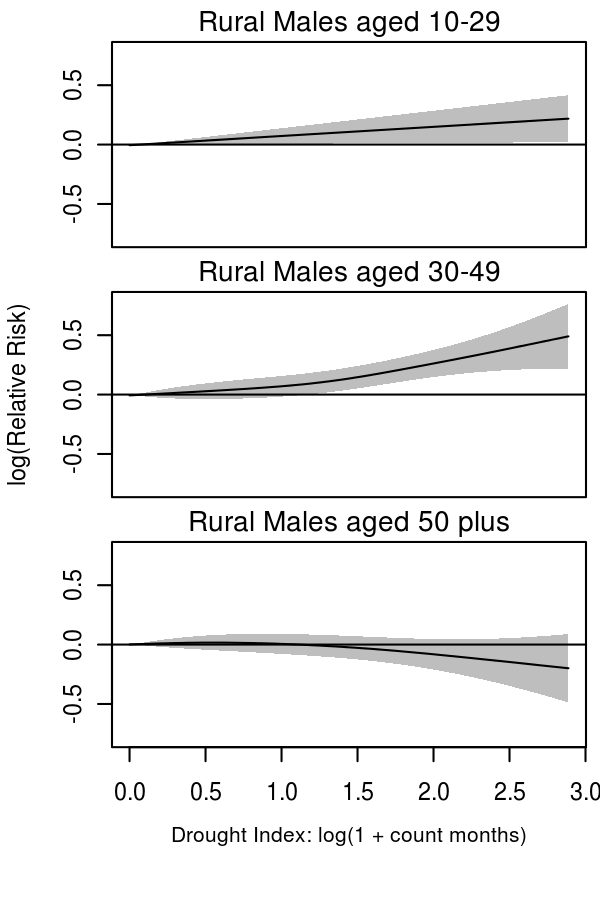
\includegraphics[width=.45\textwidth]{Figure1.png}
\caption{Figure1.png}
\label{fig:Figure1.png}
\end{figure}
\end{frame}
\section{Discussion}
\label{sec-4}
\begin{frame}
\frametitle{Criticism}
\label{sec-4-1}

This model is too static, reductionist, reality is more complex. Need to work more on interactions with non-climate factors especially: 
\begin{itemize}
\item Natural capital
\item Financial capital
\item Social capital
\item Physical capital and
\item Human capital
\end{itemize}
\end{frame}
\section{Conclusion}
\label{sec-5}
\begin{frame}
\frametitle{Conclusion}
\label{sec-5-1}

\begin{itemize}
\item Drought is related to increased suicide risk in Australia
\item Future Drought associated deaths can be calculated
\item These estimates will be very uncertain, contentious and difficult to justify
\item Data management and analysis technology such as that presented is needed to enable rigorous and transparent exploration
\end{itemize}
\end{frame}
\begin{frame}
\frametitle{Conclusion}
\label{sec-5-2}

This system:
\begin{itemize}
\item Enables data analysis in a safe environment
\item Allows comparison of multiple climate scenarios and assumptions
\item Demonstrated with a Climate/Health Impact Assessment
\item This is Reproducible
\end{itemize}
\end{frame}
\section{Acknowledgements}
\label{sec-6}
\begin{frame}
\frametitle{Acknowledgements}
\label{sec-6-1}


\includegraphics[width=4cm]{ANU_LOGO_cmyk_56mm.png}

\includegraphics[width=2cm]{andslogo.pdf}

\includegraphics[width=3cm]{deptlogo.pdf} \\
\begin{footnotesize}
This project is supported by the Australian National Data Service through the National Collaborative Research Infrastructure Strategy Program and the Education Investment Fund (EIF) Super Science Initiative.

More information from \texttt{ivan.hanigan@gmail.com} or at \texttt{[[http://opensoftware-restricteddata.github.io][http://opensoftware-restricteddata.github.io]]}

\end{footnotesize}
\end{frame}
\section{References}
\label{sec-7}
\begin{frame}
\frametitle{References}
\label{sec-7-1}

\begin{footnotesize}
\begin{thebibliography}{1}

\bibitem{Peng2011}
Roger~D Peng.
\newblock {Reproducible research in computational science.}
\newblock {\em Science (New York, N.Y.)}, 334(6060):1226--7, December 2011.

\bibitem{Hanigan2012b}
I.~C. Hanigan, C.~D. Butler, P.~N. Kokic, and M.~F. Hutchinson.
\newblock {Suicide and drought in New South Wales, Australia, 1970-2007}.
\newblock {\em Proceedings of the National Academy of Sciences}, pages
  1112965109--, August 2012.

\bibitem{Climate2008}
Hilary~J Bambrick, Keith B~G Dear, RE~Woodruff, Ivan~Charles Hanigan, and
  Anthony~J McMichael.
\newblock {The impacts of climate change on three health outcomes:
  temperature-related mortality and hospitalisations, salmonellosis and other
  bacterial gastroenteritis, and population at risk from dengue.}
\newblock Technical report, Garnaut Climate Change Review, Canberra, 2008.

\end{thebibliography}
\end{footnotesize}
\end{frame}

\end{document}
